% Author: PokMan Ho
% Script: method.tex
% Desc: MRes thesis methods section
% Input: none
% Output: none
% Arguments: 0
% Date: Apr 2020

\documentclass[../thesis.tex]{subfiles} %% use packages & commands as this main file

\begin{document}
\section{Methodology}

\subsection{the ODE model}
The minimalist model used was composed by two players/ecological engines and three finite carbon pools (Fig.\ref{modelInWord}).  Phytoplanktons (P) and bacterial decomposers (B) were the two engines powering the interactions.  The engines themselves did not contain carbon under the model's logic and only consist of cellular biochemical reactions.  Both engines were sharing all but one different link, which is where they get carbon.  P gained carbon from the external unlimited carbon pool (i.e. $CO_2$) while B gained from the finite organic carbon (C) pool.  Both engines respired, leaked carbon and allocated the rest to its biomass carbon pool.  Also, biomass pools contained fatalities and those portions were fed into the C pool along with the leaked carbon.  At the C pool, carbon could either being ingested by B or removed from the system (artificially).  The whole system would be an independent open ecosystem if the (artificial) removal flux tuned to zero.  Several assumptions were made in this project, including: 1. living conditions in the system was homogeneous spatially, nutritionally, carbon and light availability; 2. nutrient supply was continuous and unlimited by utilization of sewage;\autocite{markou2014microalgal} 3. the effect of high carbon density blocking light within the system was negligible; and 4. dissolved organic matter and dead cells provided similar growth effect on decomposers.  In short, this model had only one environmental limitation -- living space for phytoplanktons.

\begin{figure}[H]
    \centering
    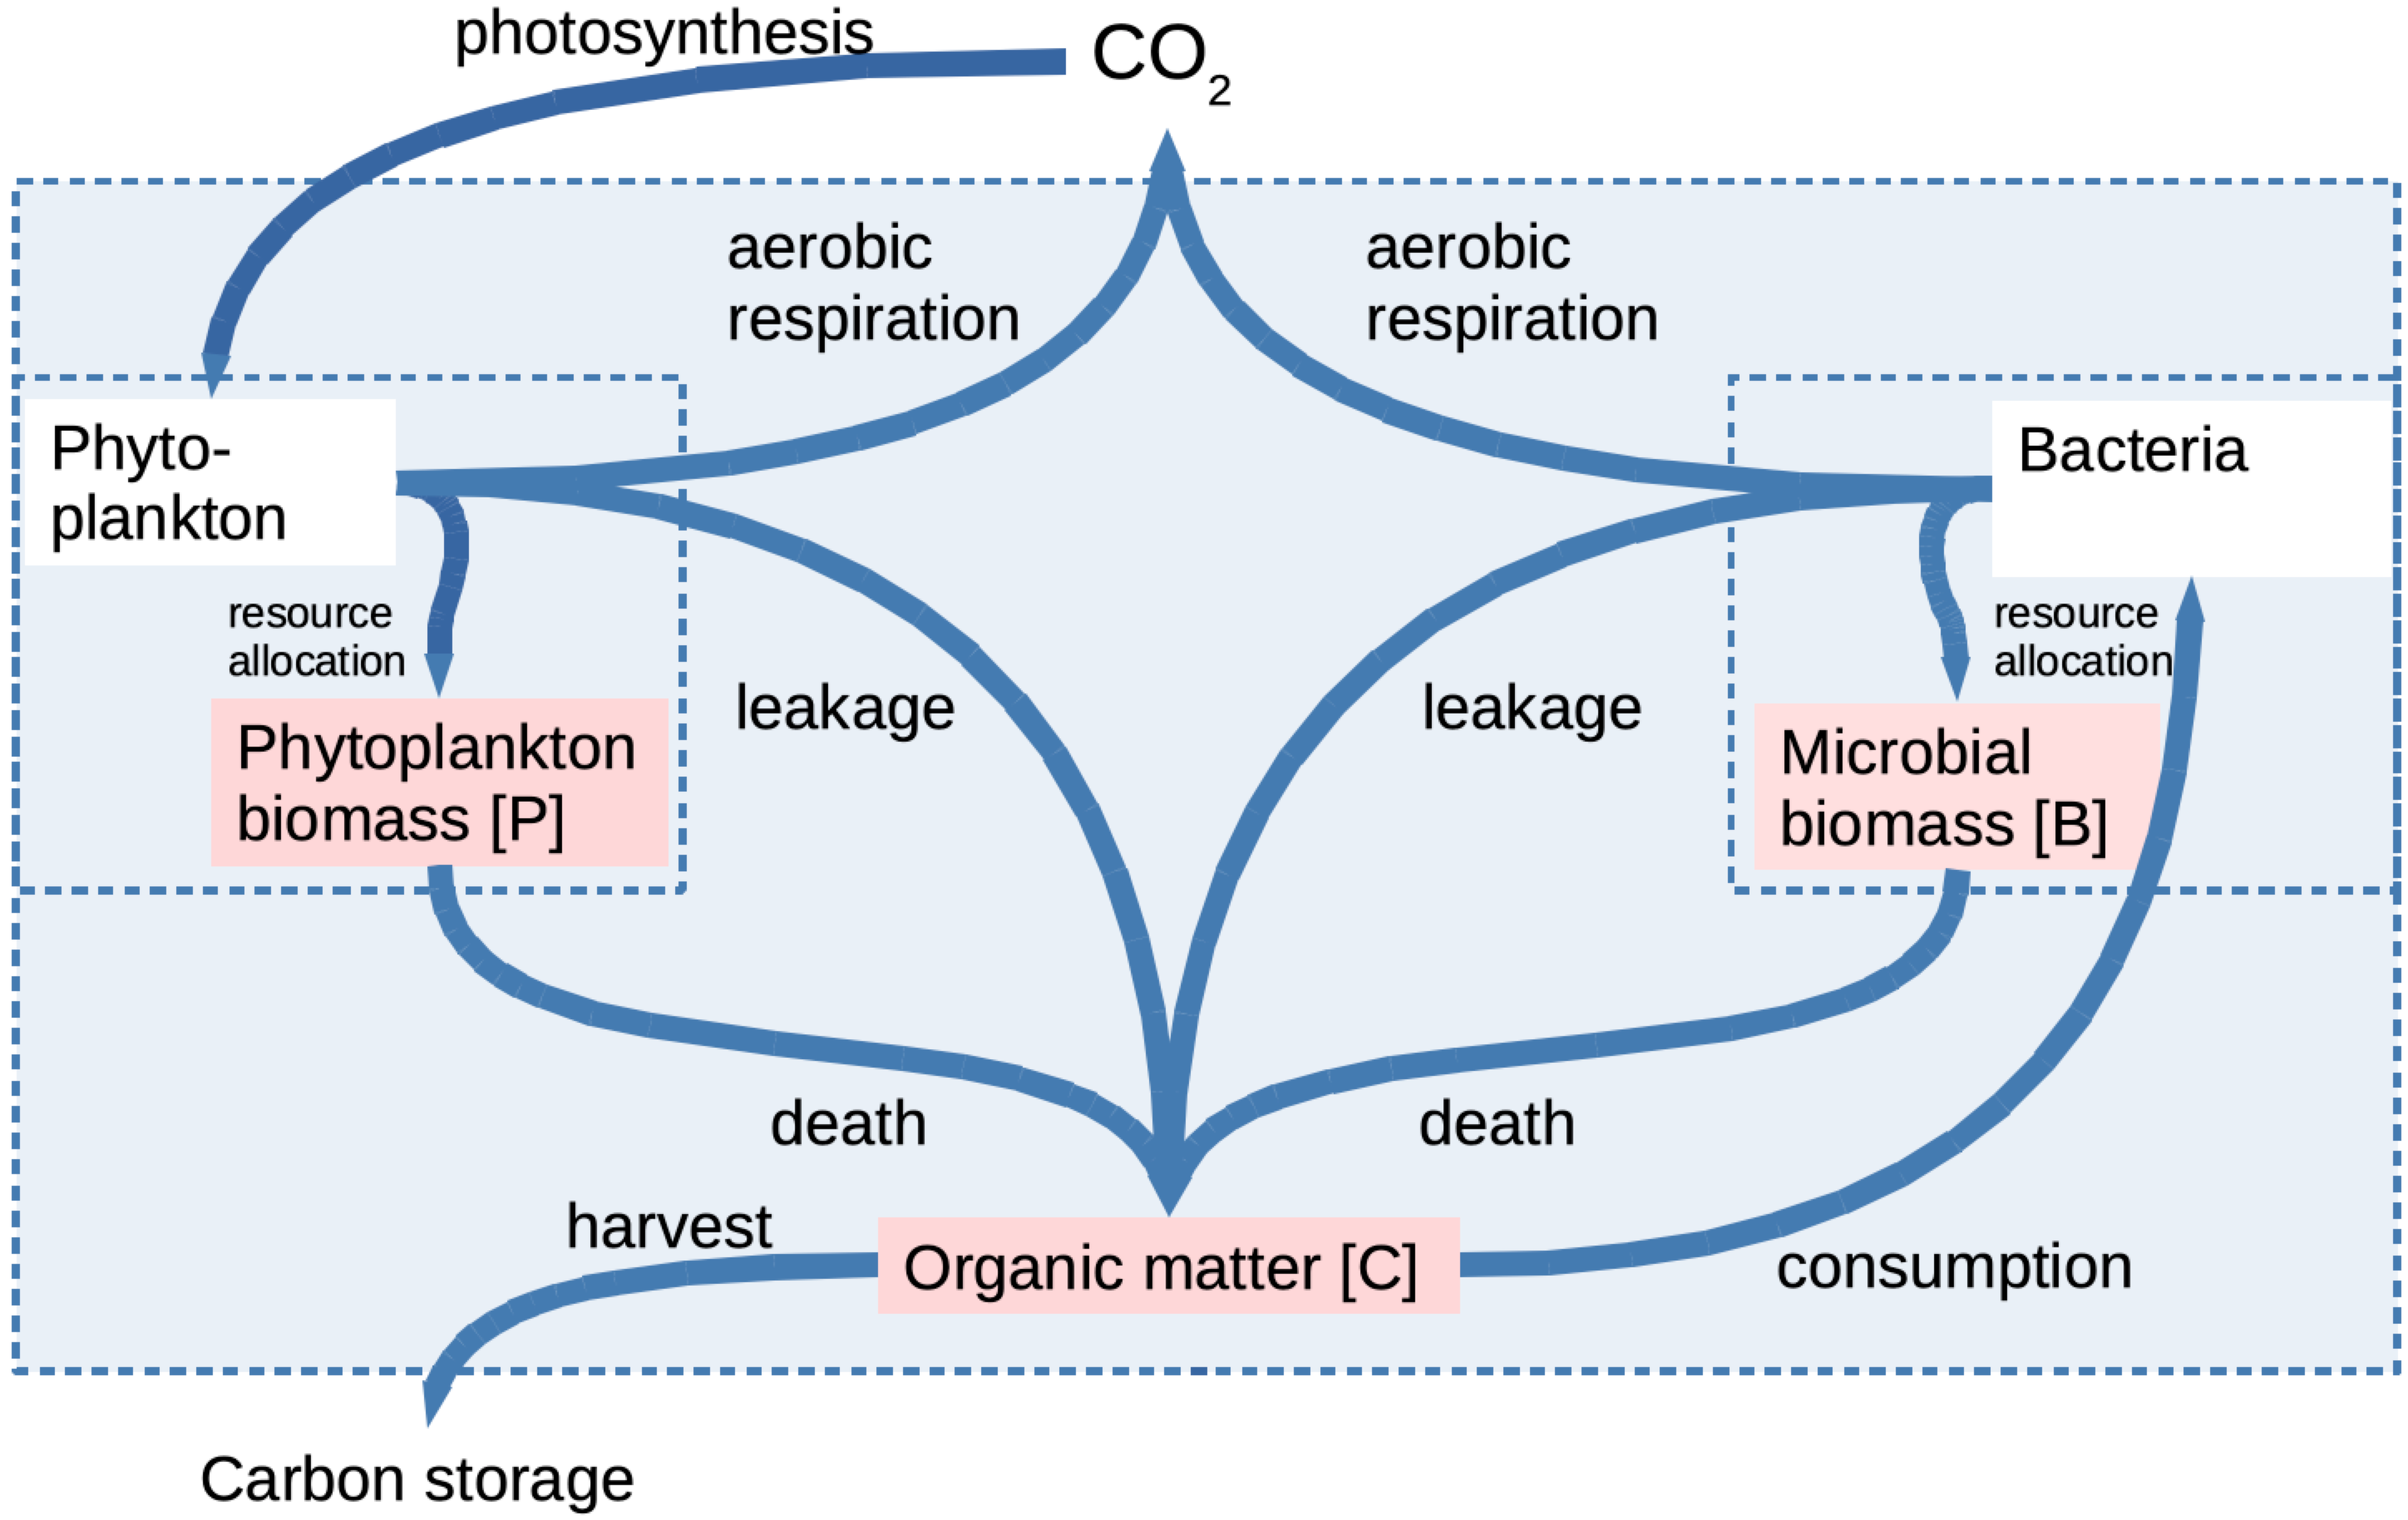
\includegraphics[width=.8\linewidth]{media/model.png}
    \caption[Model visualization]{Classification of dominant interactions in this project.  The two players shared all interactions with respective carbon pools but one, which was the energy acquiring method.}
    \label{modelInWord}
\end{figure}

\subsection{variables in the model}
Nine parameters were used to describe the system, two sets of four biological parameters for the players P and B plus one carbon removal rate parameter.  Due to the parameter values obtained, the finest time scale of this model was set as ``day".  $\ePR$ and $\eBR$ were non-respired carbon fractions for P and B respectively.  $\eP$ and $\eB$ were carbon fractions incorporated into biomass for P and B respectively.  These two fractions were unit-less and modeled using different parameters because experimentally these numbers were measured using different methods.  $\gP$ and $\gB$ were specific growth rates for P and B with different units.  Due to the model being an open system, $\gP$ only depended on P because the interacting counterpart was assumed being unlimited.  However, a finite resource pool C had made $\gB$ depended on both the resource (i.e. C) and consumer (i.e. B) density.  In this project, since it was assumed that the environment was homogeneous, $\gB$ was logically sounded to take units rate ($t^{-1}$) and rate per unit density($m^3/(gCt)$) as equivalent.  Death rates in the model were logically different between P and B.  $\aP$ was a mechanistic death term for P based on intraspecific interference, one of the reasons leading to carrying capacity.  On a contrary, $\mB$ was a simple specific death rate for B.  Hence this model had an intrinsic assumption, which assumed the only limiting factor for P was competition (the intraspecific interference) while that for B was the carbon resource availability.  Detailed version of calculating some parameters (including temperature standardisation procedures) was in the Appendix.

\begin{table}[H]
    \centering
    \caption[Algebra variables]{Table showing variables and corresponding values used in the ODE system}
    \begin{tiny}
    \csvautotabular[]{media/varTab.csv}
    \end{tiny}
    \label{varInTab}
\end{table}

\subsection{the model in equations}
Using the parameters defined in Table \ref{varInTab}, linkages in Fig.\ref{modelInWord} could be expressed in mathematical terms listed in Table \ref{termInTab}.  By considering the arrow directions (which carbon pool gained carbon and which respective pool lost), terms were grouped into three ODEs (summarised in Eqn.\ref{eq:ode}).

\begin{table}[H]
    \centering
    \caption[Processes in algebra terms]{Table showing processes in Fig.\ref{modelInWord} direct translation into mathematical terms}
    \csvautotabular[]{media/termTab.csv}
    \label{termInTab}
\end{table}

\begin{equation}\left\{\begin{array}{rl}
    C'(t) &= \ePR(1-\eP)\cdot\gP\cdot P +\aP\cdot P^2 +(\eBR(1-\eB)-1)\cdot\gB\cdot C\cdot B +\mB\cdot B -xC\\
    P'(t) &= \ePR\cdot\eP\cdot\gP\cdot P -\aP\cdot P^2\\
    B'(t) &= \eBR\cdot\eB\cdot\gB\cdot C\cdot B -\mB\cdot B
\end{array}\right.\label{eq:ode}\end{equation}

\subsection{solving the model}
Solving the ODE system analytically (i.e. integration by SciPy (v.1.4.1) ``odeint" function) showed a stable equilibrium mostly regardless to the initial value.  Solving the ODE system numerically (setting $\dC=\dP=\dB=0$ and solve the system of unknowns by SymPy (v.1.0.7) in Julia-lang (v.1.3.1)) revealed four alternative equlibrium positions but only one of them contained all non-zero three carbon pools densities (coexistence equilibrium).  When comparing the analytical result with the coexistence equilibrium using parameter values within the ranges in Table\ref{varInTab}, both methods gave similar equilibria values (converged to 2 d.p.).

The coexistence equilibrium is solved as
\begin{equation}\left\{\begin{array}{rl}
    C &= \dfrac{\mB}{\eBR\eB\gB}\\
    P &= \dfrac{\ePR\eP\gP}{\aP}\\
    B &= \dfrac{\aP\mB x-\eBR\eB\gB\eP(\ePR\gP)^2}{\gB\mB\aP(\eBR-1)}
\end{array}\label{eq:solC}\text{, when }\dC=\dP=\dB=0
\right.\end{equation}

It is logical to conclude the validity of using this set of carbon pool solution to get rapid detection of coexistence on the ODE system across designated parameter spaces (Table \ref{varInTab}).

\subsection{analysis}

\end{document}
